%!TEX program = xelatex
% 完整编译: xelatex -> bibtex -> xelatex -> xelatex
\documentclass[lang=cn,a4paper,cite=authoryear]{elegantpaper}
\songti

\title{\zihao{1}哈尔滨工业大学计算机科学与技术学院 \par 实验报告}
\date{}
% 本文档命令
\usepackage{array}
\usepackage{graphicx}
\usepackage{minted}
\usepackage{subfigure}
\usepackage{enumitem}
\newcommand{\ccr}[1]{\makecell{{\color{#1}\rule{1cm}{1cm}}}}

\begin{document}

\maketitle
\thispagestyle{empty}
\begin{center}
	\zihao{3}
   	{ 课程名称:  机器学习}\\[.5cm]
    { 课程类型:   选修}\\[.5cm]
    { 实验题目:  实现k-means聚类方法和混合高斯模型}\\[.5cm]
	{ 学 号:  1190202110}\\[.5cm]
	{ 姓 名: 田雪洋}\\[.5cm]
    { \date{\zhtoday}}\\[.50cm]
\end{center}


\newpage
\zihao{4}
\section*{\zihao{2}{一、实验目的}}
实现一个k-means算法和混合高斯模型,并且用EM算法估计模型中的参数。

\section*{\zihao{2}{二、实验要求及实验环境}}
\subsection*{\zihao{-2}{1.实验要求}}
目标:实现一个k-means算法和混合高斯模型,并且用EM算法估计模型中的参数。

\par 测试:
\par 用高斯分布产生k个高斯分布的数据(不同均值和方差)(其中参数自己设定)。
\par(1)用k-means聚类,测试效果;
\par(2)用混合高斯模型和你实现的EM算法估计参数,看看每次迭代后似然值变化情况,考察EM算法是否可以获得正确的结果(与你设定的结果比较)。

\par 应用:可以UCI上找一个简单问题数据,用你实现的GMM进行聚类。


\subsection*{\zihao{-2}{2.实验环境}}
Windows10; python3.8.6;Pycharm 
\section*{\zihao{2}{三、设计思想(本程序中的用到的主要算法及数据结构)}}
\subsection*{\zihao{-2}{1.k-means算法}}
聚类的对象是观测数据的集合。假设有n个样本,每个样本由m个属性的特征向量组成。样本集合可以表示为矩阵X:
$$
X=\left[ x_{ij} \right] _{m\times n}=\left[ \begin{matrix}
	x_{11}&		x_{12}&		\cdots&		x_{1n}\\
	x_{21}&		x_{22}&		\cdots&		x_{2n}\\
	\vdots&		\vdots&		\ddots&		\vdots\\
	x_{m1}&		x_{m2}&		\cdots&		x_{mn}\\
\end{matrix} \right] 
$$
矩阵的第$j$列表示为第$j$个样本,$j=1,2,...,n$;第$i$行表示为第$i$个属性,$i=1,2,...,m$。
\par K-means算法的聚类过程如下:
\begin{enumerate}[(1)]
	\item 初始化。令$t=0$,随机选取k个样本点作为初始聚类的中心$m^{\left( 0 \right)}=\left( m_{1}^{\left( t \right)},\cdots m_{l}^{\left( t \right)},\cdots ,m_{k}^{\left( t \right)} \right) $
	\item E步:
	对于每一个样本i,计算其应该属于的类,使得损失函数极小化,结果构成聚类$C^{\left( t \right)}$:
	$$
	\min_C \sum_{l=1}^k{\sum_{C_{}^{\left( t \right)}\left( i \right) =l}^{}{\left\| x_i-m_{l}^{\left( t \right)} \right\| ^2}}
	$$
	\par 即,在类中心确定的情况下,将样本分到一个类中,使得样本和其所属类的中心之间的距离总和最小。
	\item M步:
     计算新的类中心,对于聚类结果$C^{\left( t \right)}$,计算当前各个类中的样本均值,作为新的类别中心$m^{\left( t+1 \right)}=\left( m_{1}^{\left( t+1 \right)},\cdots m_{l}^{\left( t+1 \right)},\cdots ,m_{k}^{\left( t+1 \right)} \right) $:
	\par
	$$
	m_{l}^{\left( t+1 \right)}=\frac{1}{n_l}\sum_{C^{\left( t+1 \right)}\left( i \right) =l}{x_i}
	$$
\end{enumerate}

\subsection*{\zihao{-2}{2.混合高斯模型}}
聚类的对象是观测数据的集合。假设有n个样本,每个样本由m个属性的特征向量组成。样本集合可以表示为矩阵X:
$$
X=\left[ x_{ij} \right] _{m\times n}=\left[ \begin{matrix}
	x_{11}&		x_{12}&		\cdots&		x_{1n}\\
	x_{21}&		x_{22}&		\cdots&		x_{2n}\\
	\vdots&		\vdots&		\ddots&		\vdots\\
	x_{m1}&		x_{m2}&		\cdots&		x_{mn}\\
\end{matrix} \right] 
$$
矩阵的第$j$列表示为第$j$个样本,$j=1,2,...,n$;第$i$行表示为第$i$个属性,$i=1,2,...,m$。
则对于上述$n$维空间中的随机变量$x_j$服从多元高斯分布,其概率密度函数为:
\begin{equation}
	p(\mathbf{x} \mid \mu, \Sigma)=\frac{1}{(2 \pi)^{\frac{n}{2}}|\Sigma|^{\frac{1}{2}}} \exp \left(-\frac{1}{2}(\mathbf{x}-\mu)^{T} \Sigma^{-1}(\mathbf{x}-\mu)\right)
\end{equation}
其中$\mu$是n维均值向量,$\Sigma$是$n*n$的协方差矩阵。则由其生成的高斯混合混合分布为:
\begin{equation}
	p_{\mathcal{M}}=\sum_{i=1}^{k} \alpha_{i} p\left(\mathbf{x} \mid \mu_{\mathbf{i}}, \Sigma_{i}\right)
\end{equation}
该分布由k个高斯分布组成,其中$\mu_i$和$\Sigma_i$是第i个高斯分布的参数。且$\aleph_i>0,\sum_{i=1}^{k} \alpha_{i}=1$。
令随机变量$z_j$为生成样本$x_j$的高斯混合成分。显然$z_j$的取值未知,但$z_j$的先验概率$P(z_j=j)=\alpha_{j}$,那么由贝叶斯定理得$z_j$的后验分布为:
\begin{equation}
	p_{\mathcal{M}}\left(z_{j}=i \mid \mathbf{x}_{\mathbf{j}}\right)=\frac{p\left(z_{j}=i\right) \cdot p_{\mathcal{M}}\left(\mathbf{x}_{\mathbf{j}} \mid z_{j}=i\right)}{p_{\mathcal{M}}\left(\mathbf{x}_{\mathbf{j}}\right)}=\frac{\alpha_{i} \cdot p\left(\mathbf{x}_{\mathbf{j}} \mid \mu_{\mathbf{i}}, \Sigma_{i}\right)}{\sum_{l=1}^{k} \alpha_{l} p\left(\mathbf{x}_{\mathbf{j}} \mid \mu_{\mathbf{1}}, \Sigma_{l}\right)}
\end{equation}
则,当高斯混合分布已知时,高斯混合聚类将把样本集X划分为k个簇$C={C_1,C_2,...,C_k}$。每个样本$x_j$的簇标记$\lambda_j$为:
\begin{equation}
	\lambda_{j}=\arg \max _{i} p_{\mathcal{M}}\left(z_{j}=i \mid \mathbf{x}_{\mathbf{j}}\right)
\end{equation}
对于模型参数$\left\{\alpha_{i}, \mu_{i}, \Sigma_{i} \mid i \in\{1,2, \ldots, k\}\right\}$的求解,则采用极大似然估计,则其极大似然函数为:
\begin{equation}
	L L(D)=\ln \left(\prod_{j=1}^{m} p_{\mathcal{M}}\left(\mathbf{x}_{\mathbf{j}}\right)\right)=\sum_{j=1}^{m} \ln \left(\sum_{i=1}^{k} \alpha_{i} \cdot p\left(\mathbf{x}_{\mathbf{j}} \mid \mu_{i}, \Sigma_{i}\right)\right)
\end{equation}
然后(5)式对$\mu_{i}$,$\Sigma_{i}$分别求偏导数,并令偏导数等于0,得到:
\begin{equation}
	\mu_{i}=\frac{\sum_{j=1}^{m} p_{\mathcal{M}}\left(z_{j}=i \mid \mathbf{x}_{\mathbf{j}}\right) \cdot \mathbf{x}_{\mathbf{j}}}{\sum_{j=1}^{m} p_{\mathcal{M}}\left(z_{j}=i \mid \mathbf{x}_{\mathbf{j}}\right)}
\end{equation}
\begin{equation}
	\Sigma_{i}=\frac{\sum_{j=1}^{m} p_{\mathcal{M}}\left(z_{j}=i \mid \mathbf{x}_{\mathbf{j}}\right) \cdot\left(\mathbf{x}_{\mathbf{j}}-\mu_{\mathbf{i}}\right)\left(\mathbf{x}_{\mathbf{j}}-\mu_{\mathbf{i}}\right)^{T}}{\sum_{j=1}^{m} p_{\mathcal{M}}\left(z_{j}=i \mid \mathbf{x}_{\mathbf{j}}\right)}
\end{equation}
对于混合系数$\alpha_i$,不仅要最大化(5)式,还要满足$\aleph_i>0,\sum_{i=1}^{k} \alpha_{i}=1$。因此考虑(5)式的拉格朗日形式
\begin{equation}
	LL(D)+\lambda(\sum_{i=1}^{k} \alpha_{i}-1)
\end{equation}
其中$\lambda$为拉格朗日乘子,且满足$\lambda=-m$。对该式求偏导得到:
\begin{equation}
	\alpha_{i}=\frac{1}{m} \sum_{j=1}^{m} \frac{p\left(\mathbf{x}_{\mathbf{j}} \mid \mu_{i}, \Sigma_{i}\right)}{\sum_{l=1}^{k} \alpha_{l} \cdot p\left(\mathbf{x}_{\mathbf{j}} \mid \mu_{l}, \Sigma_{l}\right)}
\end{equation}
GMM算法的聚类过程如下:
\begin{enumerate}[(1)]
\item 随机初始化参数$\{\alpha_i, \mu_i, \Sigma_i|i \in \{1, 2, \dots, k\}\}$以及$\bold{C_i} = \emptyset$
\item 开始迭代至带到迭代次数或者是参数值不再发生变化:
      \par E步:根据式$(3)$计算每个样本由各个混合高斯成分生成的后验概率
      \par M步:根据式$(6)(7)(9)$更新参数$\{\alpha_i, \mu_i, \Sigma_i|i \in \{1, 2, \dots, k\}\}$
\par 根据式$(4)$确定每个样本的簇标记$\lambda_j$,并将其加入相应的簇$\bold{C_{\lambda_j}} = \bold{C_{\lambda_j} \cup \{\bold{x_j}\}}$
\item 输出簇划分$C = \{\bold{C_1, C_2, \dots, C_k}\}$
\end{enumerate}
\section*{\zihao{2}{四、实验结果与分析}}
\subsection*{\zihao{-2}{1.生成数据}}
首先,为了方便可视化展现实验结果,本次实验选取二维高斯分布,并生成了三个二维高斯簇,进行测试。在这里,由于本次实验,事先知道每一个点所属的类别,因此,将分类后求出的类别,和已知类别进行对比,可以求出定义聚类准确率。

\subsection*{\zihao{-2}{2.K-means}}
使用K-means算法得到的实验结果如下:
\begin{center}
	\begin{figure}[H]
		\centering
		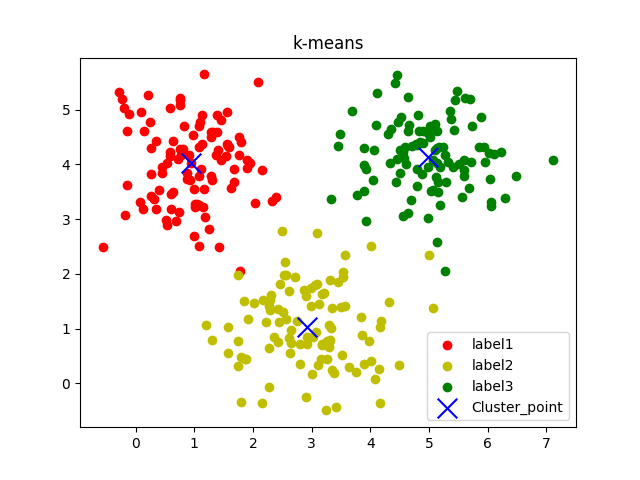
\includegraphics[scale=0.6]{figure_1}
	\end{figure}
\end{center}
可以看到,K-means算法可以很好地划分出不同的聚类簇,并且求出的簇中心的位置很合理。准确率为:99.3\% 。

\subsection*{\zihao{-2}{3.GMM}}
使用GMM算法得到的实验结果如下:
\begin{center}
	\begin{figure}[H]
		\centering
		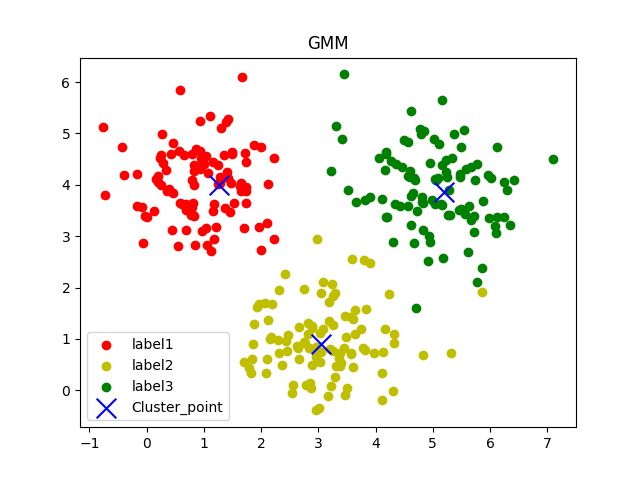
\includegraphics[scale=0.6]{figure_2}
	\end{figure}
\end{center}
可以看到,GMM算法可以很好地划分出不同的聚类簇,并且求出的簇中心的位置很合理。准确率为:94\% 。
\par
K-means算法和GMM算法法在生成数据上的表现类似,都可以很高效准确地实现聚类。
\subsection*{\zihao{-2}{3.UCI数据集}}
UCI数据集中的iris数据集是简单经典的用于分类任务和聚类任务的数据集。本次实验采用iris数据集进行聚类任务测试。本次实验首先对鸢尾花数据集的标签数字化,经分析,选取petal\_length和petal\_width这两个特征进行聚类,K-means算法和GMM算法的结果分别如下:
\par 使用K-means算法得到的实验结果如下:
\begin{center}
	\begin{figure}[H]
		\centering
		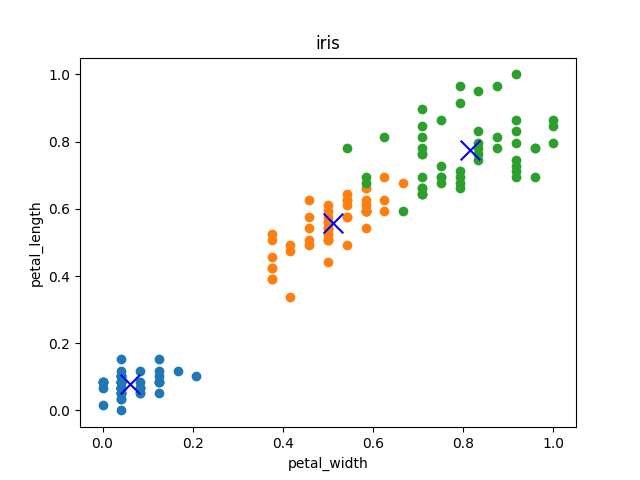
\includegraphics[scale=0.6]{figure_3}
	\end{figure}
\end{center}
可以看到,K-means算法可以很好地划分出不同的聚类簇,并且求出的簇中心的位置很合理。准确率为:96\% 。

\par 使用GMM算法得到的实验结果如下:
\begin{center}
	\begin{figure}[H]
		\centering
		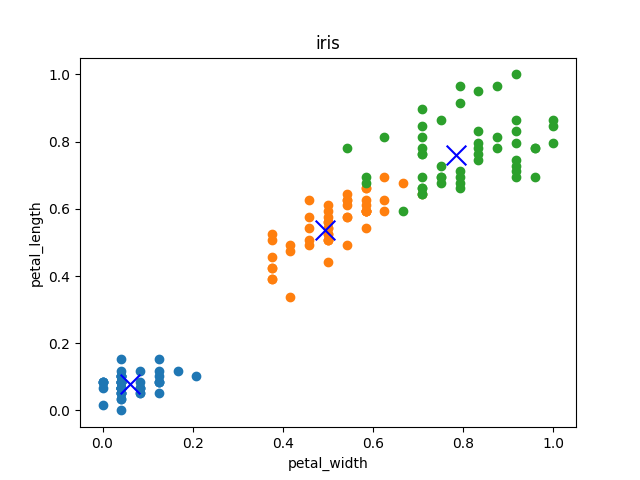
\includegraphics[scale=0.6]{figure_4}
	\end{figure}
\end{center}
可以看到,GMM算法可以很好地划分出不同的聚类簇,并且求出的簇中心的位置很合理。准确率为:98\% 。
\par 在实际数据集上,本实验算法依然能够很好地完成聚类任务。
\section*{\zihao{2}{五、结论}}
\begin{itemize}
	\item  K-means算法利用欧式距离来衡量样本与各个簇中心的相似程度
	\item K-Means的簇中心初始化对于最终的结果有很大的影响,如果选择不好初始的簇中心值容易使之陷
	入局部最优解
	\item GMM使用EM算法进行迭代优化,因为其涉及到隐变量的问题,是在不完全数据上进行的聚类。
	\item EM算法具备收敛性,但并并不一定找到全局最大值,有可能只能找到局部最大值。
\end{itemize}
\section*{\zihao{2}{六、参考文献}}
\begin{enumerate}[(1)]
	\item  周志华 著. 机器学习, 北京: 清华大学出版社, 2016.1
	\item  李航 著. 统计学习方法,北京:清华大学出版社,2020.6
\end{enumerate}
\section*{\zihao{2}{七、附录:源代码(带注释)}}
源代码见相关文件
\begin{enumerate}[(1)]
	\item  data\_process.py:数据预处理,生成,计算准确率
	\item  GMM.py:实现GMM算法
	\item  k\_means.py:实现K-means算法
	\item  testOf\_GMM.py:利用生成数据测试GMM算法,并绘图
	\item  testOfK\_means.py 利用生成数据测试K-means算法,并绘图
	\item  iris\_GMM.py:利用鸢尾花数据测试GMM算法,并绘图
	\item  iris\_k\_means.py 利用鸢尾花数据测试K-means算法,并绘图
\end{enumerate}
\end{document}